\begin{section}{GP}{Constraining feedback models due to the number of baryons \\
   in the circumgalactic medium (CGM)}
  \begin{minipage}{\linewidth}
    \begin{wrapfigure}{r}{0pt}
      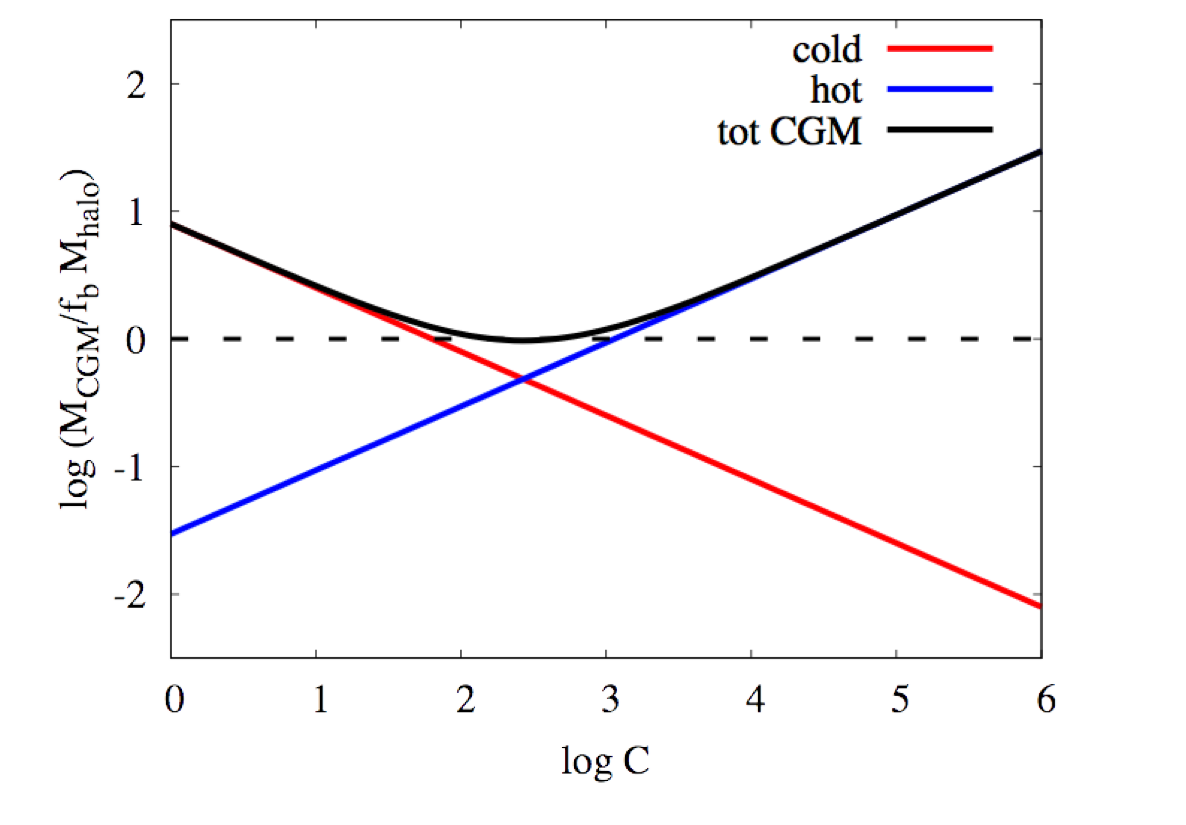
\includegraphics[width=15cm]{GP/fig1.png}
    \end{wrapfigure}
    \strut {\small Mass of the CGM in our model of the MUSE Giant Ly$\alpha$
      nebulae (in units of the maximum baryon mass $(\Omega_b/\Omega_m)M_h$,
      marked as a horizontal dashed line), as a function of the clumping factor
      of the cold gas, assuming fiducial values for halo mass and cold gas
      temperature of $M_h = 10^{12.3} M_{\odot}$ and $T=2 \times 10^4 K$. The
      red, blue and black lines are for the cold, hot and total gas,
      respectively. Viable models require a clumping factor $C \approx 300$ and
      a total baryon fraction very close to the cosmological value.}
  \end{minipage}

  \vspace{0.7cm}

  \begin{minipage}{\linewidth}
    \begin{wrapfigure}{r}{0pt}
      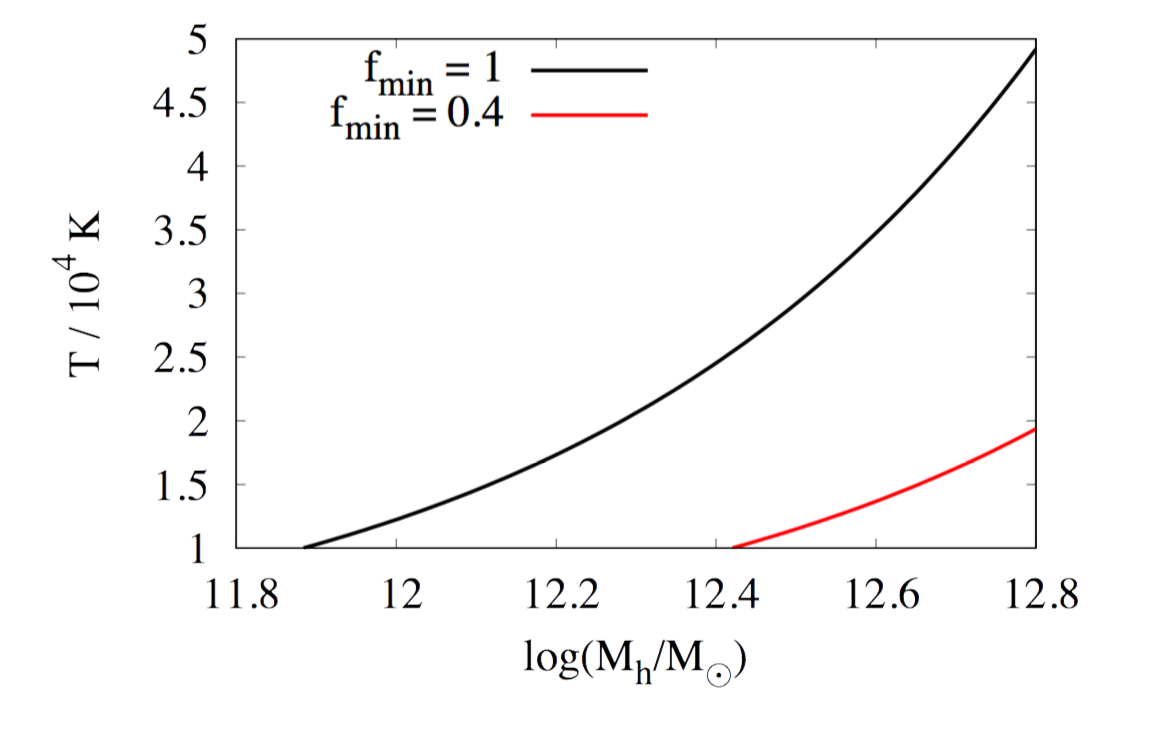
\includegraphics[width=15cm]{GP/fig2.png}
    \end{wrapfigure}
    \strut {\small Minimum total CGM baryon fraction (corresponding to
      equipartition of the the CGM into the cold and hot phases), as a function
      of the two model parameters: halo mass and temperature of the cold gas.
      Low halo masses and high temperatures are inconsistent with cosmology for
      exceeding the universal baryon fraction. Only the highest halo masses and
      the lowest gas temperatures are consistent with $f_{CGM} \leq 0.4$, as
      expected for models with strong ejective feedback at high $z$.}
  \end{minipage}
\end{section}